\chapter{Signal simulation and event selection} 
\label{chap:signalsel}

\section{\ttDM simplified models}
\label{sec:simpmodels}

The DM collider signal under investigation in this work is characterized by the production of a top quark pair recoiling against a spin-0 mediator that decays to a pair of DM particles, as shown in~\FigureRef{fig:ttDM}. As described in greater detail in~\SectionRef{sec:BSM}, the model predicts the production of DM via a scalar (S) or pseudoscalar (PS) mediator, which couples to SM fermions and the Dirac fermion DM particles. The coupling of the mediator to the top quarks is Yukawa-type hence \gq, which is effectively the multiplier to the Yukawa coupling, is taken to be unitary. Meanwhile, the direct coupling of the mediator to the DM particles, \gDM, is also equal to one.

The most important characteristic of \ttDM models is the \pt of the $\chi\bar{\chi}$ system. This quantity is equivalent to the \pt of the mediator and is translated to the \ptmiss detector observable in an event. The \ptmiss spectra for the \ttDM models, although dependent on the mediator mass, are expected to have longer ``tails'' at high \MET, than that of the SM \ttbar process, owing to the additional contribution from the $\chi\bar{\chi}$ system. In general, the mediator \pt spectrum broadens with increasing mediator mass, as demonstrated in~\FigureRef{fig:SvPSmedpt}, where the \pt is shown for various S and PS mediator masses with $\mDM=1\:\GeV$. It is also the case that at low masses, the PS \pt is harder than the S \pt of equivalent mediator mass, however the distributions converge to at higher mediator mass. The trend of broadening mediator \pt spectra with increasing mediator mass does not hold in the off-shell regime where the mediator mass is less than twice the DM fermion mass ($2\mDM > \mMed$). In the off-shell regime, the \pt of the mediator is not dependent on the mass, and in addition, if the $\mDM$ is varied for a fixed mediator mass, the \pt distribution is harder for the off-shell production rather than the on-shell. Due to the finite mediator width, in the area near the on/off-shell threshold, the kinematics will contain contributions from both types of production, as seen in~\FigureRef{fig:dmf_medpt2}. 

\begin{figure}
  \begin{center}
    \feynmandiagram[horizontal=c to h]{
      a [particle=\(\bar{t}\)] -- [fermion] b -- [fermion] c -- [fermion] d -- [fermion] e [particle=\(t\)],
      f [particle=\(g\)] -- [gluon] b,
      g [particle=\(g\)] -- [gluon] d,
      c -- [scalar, edge label=\(\phi \slash a\)] h,
      i [particle=\(\bar{\chi}\)] -- [fermion] h -- [fermion] j [particle=\(\chi\)],
      e -- [opacity=0.0001] i,
      a -- [opacity=0.0001] j,
      i -- [opacity=0.0001] j,
%%      f -- [opacity=0.0001] g,
    };
    \caption{The representative diagram of a top quark pair produced in association with a pair of DM particles ($\chi\bar{\chi}$) which are produced via a S or PS mediator coupled to the tops.}
    \label{fig:ttDM}
  \end{center}
\end{figure}

\begin{figure}[htbp!]
  \begin{center}
    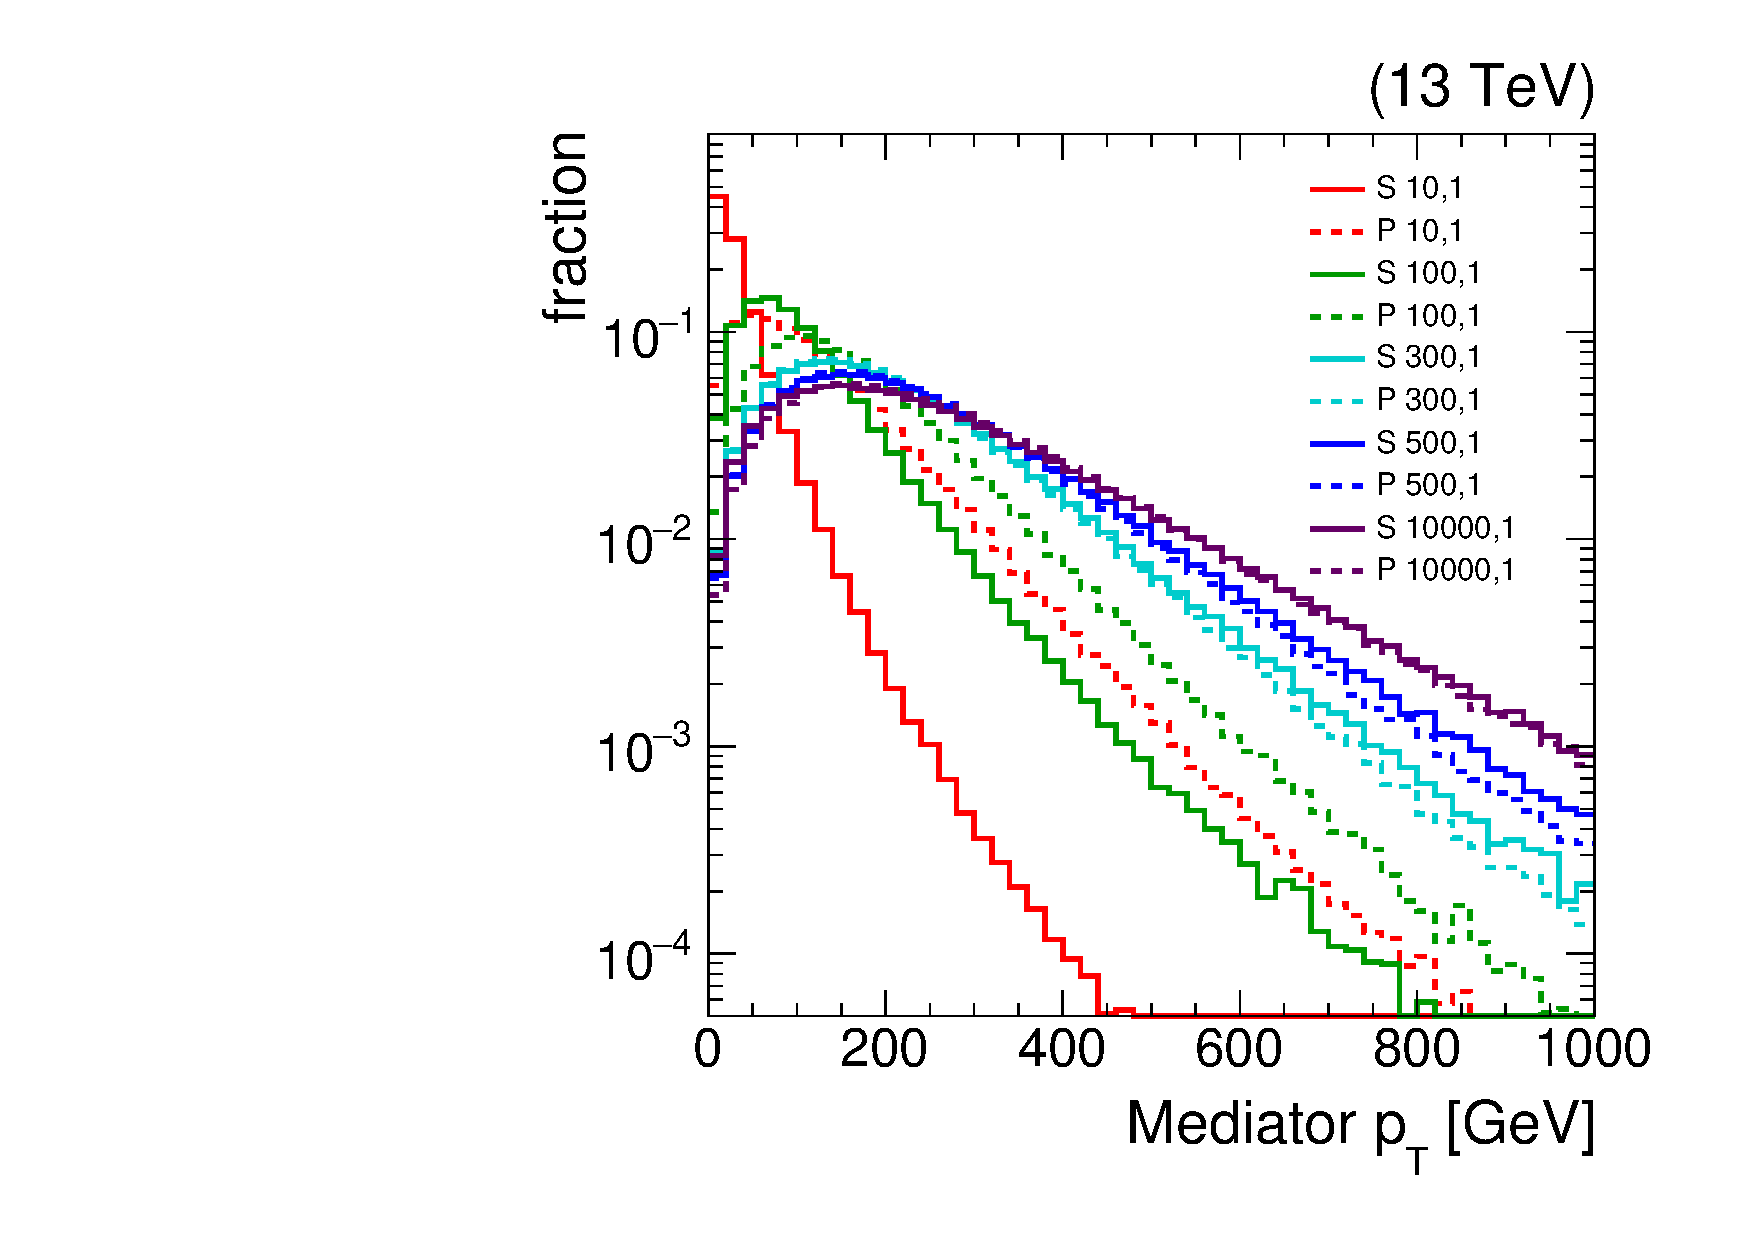
\includegraphics[width=0.48\textwidth]{figs/medptlog.pdf}
    \caption{Generator level \pt distributions for S (solid lines) and PS (dashed lines) mediators, with $\mDM=1\:\GeV$. The label ``S 10, 1'' can be understood as a model with S mediator mass $\mMed=10\:\GeV$, and DM mass $\mDM=1\:\GeV$. \pt distributions with the same color have the same mediator mass.}
    \label{fig:SvPSmedpt}
  \end{center}
\end{figure}

\begin{figure}[htbp!]
\begin{center}
  \subfloat[][]{\label{subfig:dmf_off}   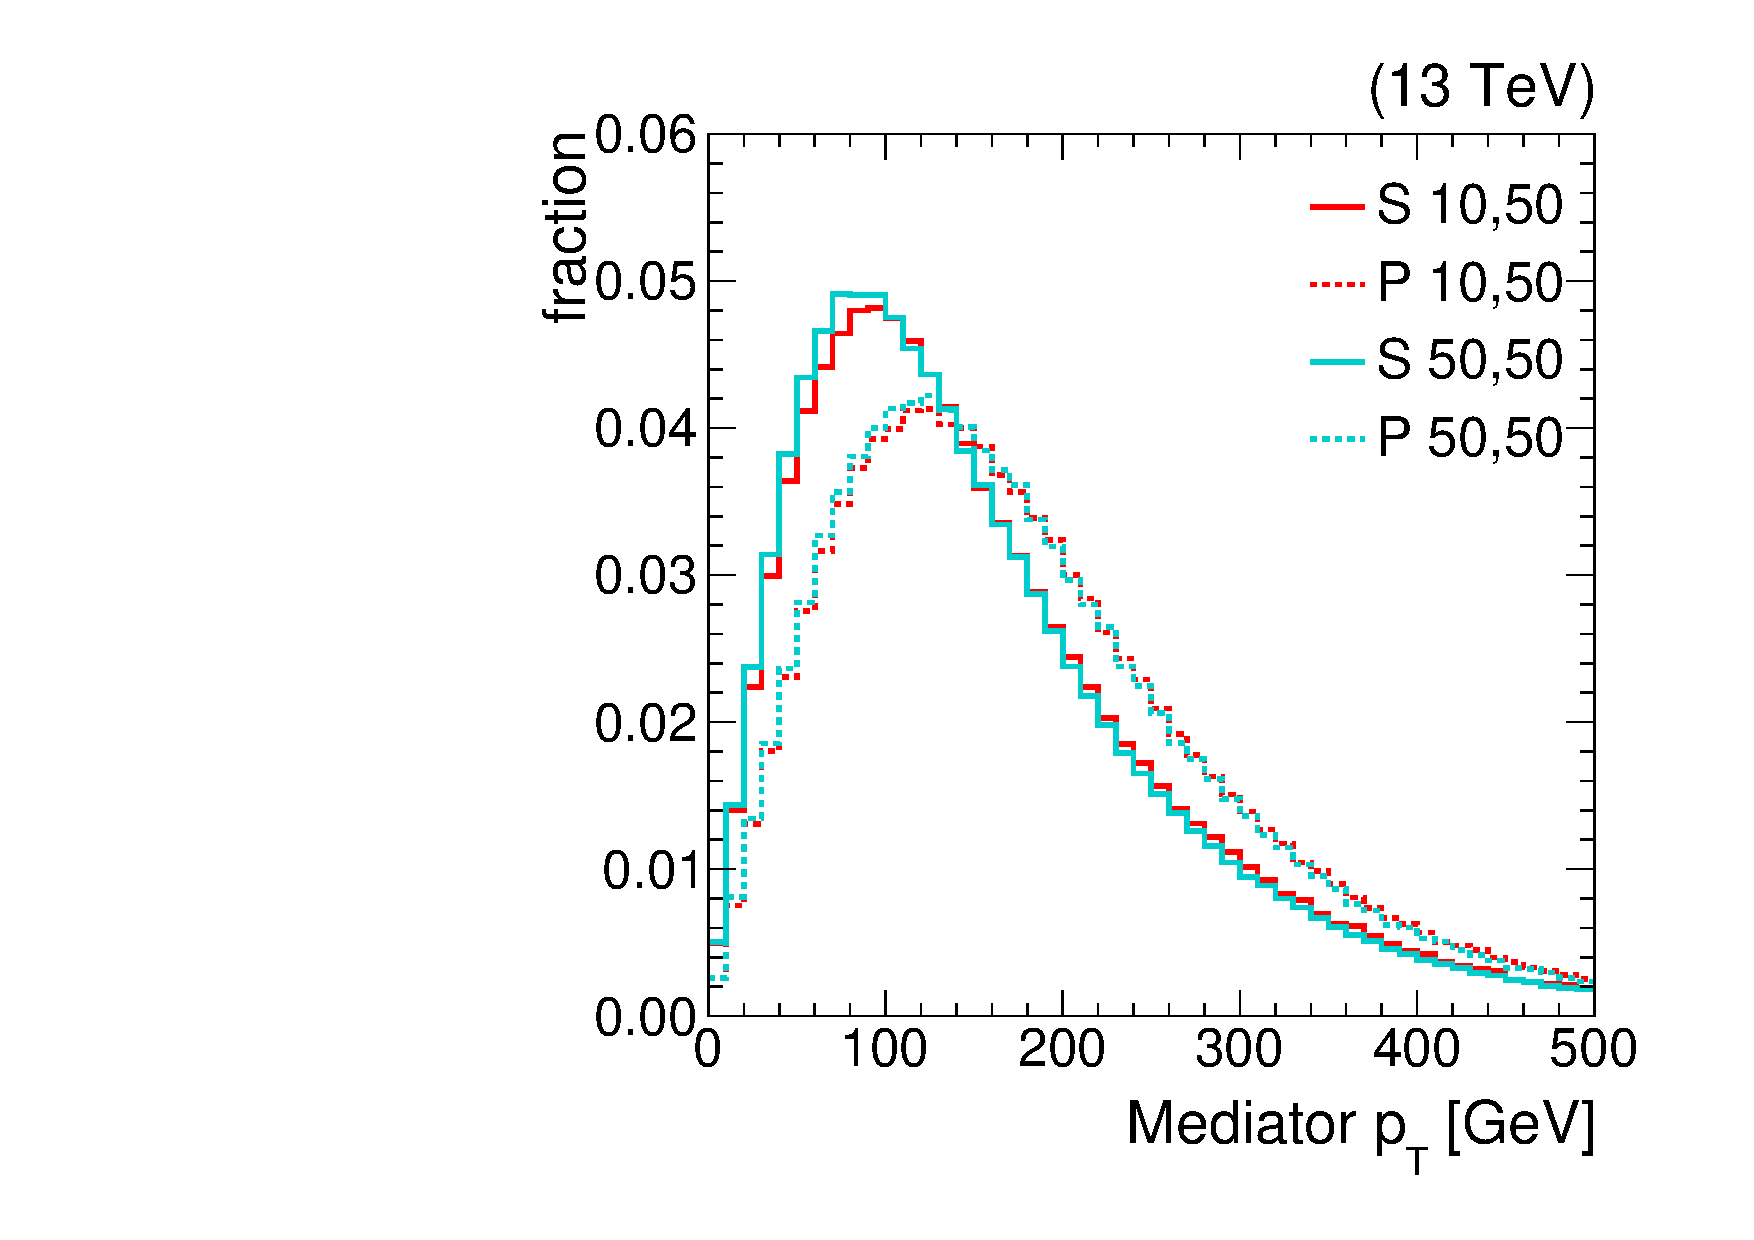
\includegraphics[width=0.48\textwidth]{figs/offshell_medpt.pdf}}
  \subfloat[][]{\label{subfig:dmf_on_off}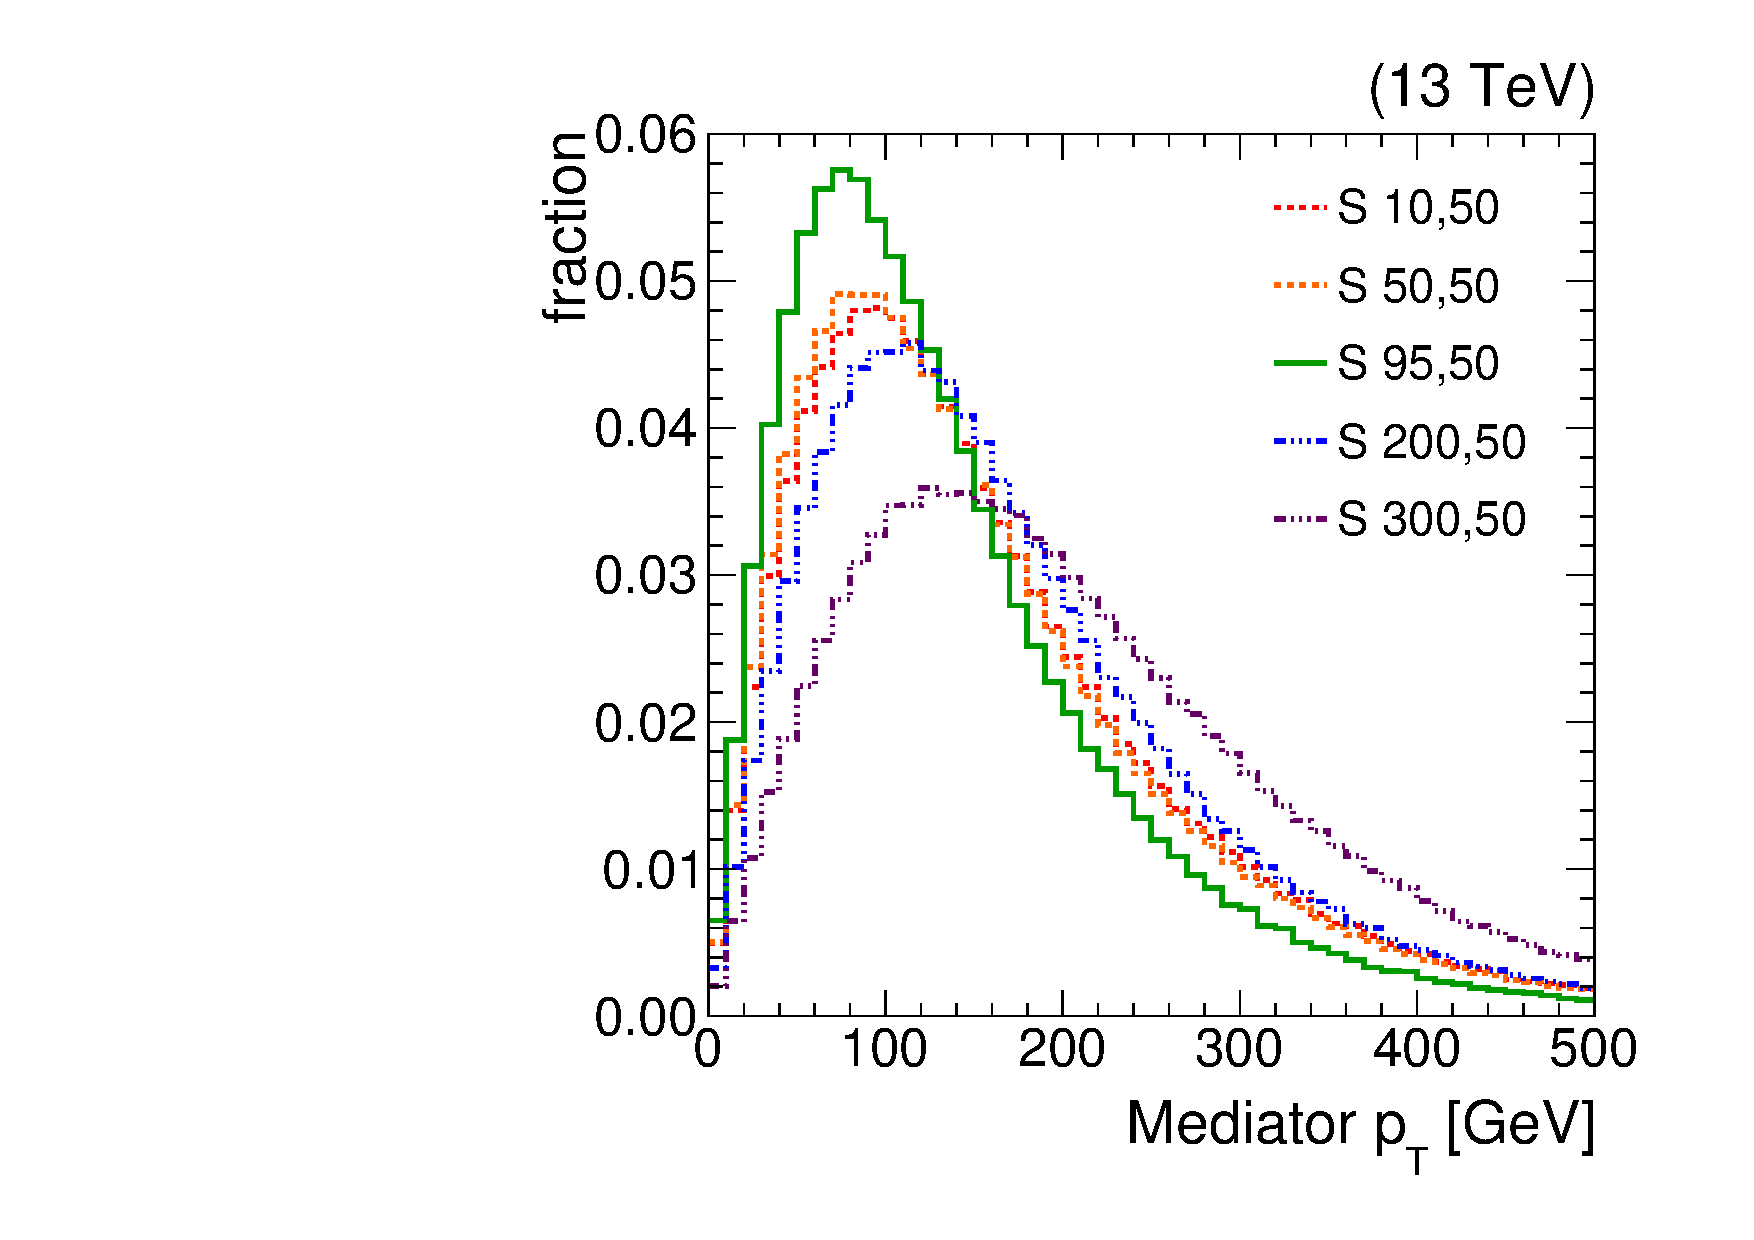
\includegraphics[width=0.48\textwidth]{figs/onshell_vs_offshell_medpt.pdf}}
  \caption{~\protect\subref{subfig:dmf_off} Generator level $\pt$ distributions for off-shell production, with solid  (dashed) lines for S (PS) mediated models, and $\mDM=50\:\GeV$. The label ``S 10, 50'' can be understood as a model with S $\mMed=10\:\GeV$ and $\mDM=50\:\GeV$. \protect\subref{subfig:dmf_on_off} Near the on-shell/off-shell threshold (green solid line), the kinematics have contributions from on-shell and off-shell production.}
  \label{fig:dmf_medpt2}
\end{center}
\end{figure}

The \ttDM signals are generated in the dilepton final state at LO accuracy in perturbative QCD using \AMCATNLO \textsc{v2.2.2}~\cite{Alwall:2014hca} with up to one additional jet, however as described in~\cite{Backovic:2015soa}, the cross section is computed at NLO with no additional partons in the Born process, and the samples are normalized to the NLO values listed in \TableRef{tab:NLOxsec}. The MLM parton-jet matching prescription~\cite{Mangano:2006rw} is used to match jets from the matrix element to the parton shower. The spin correlations in the decays of top quarks are preserved through the use of \MadSpin. The partial width formulae given in ~\cite{PhysRevD.91.055009} are used to calculate the minimum decay widths for the mediators. The calculation assumes that the mediator couples only to SM quarks and the fermion DM particle (\chi), and decays exclusively to a DM pair.  

\begin{table}
  \centering
  \begin{tabular}{|r|r|c|c|}
    \hline
    \mMed [GeV] & \mDM [GeV] & Scalar (pb) & Pseudoscalar (pb) \\
    \hline
    %% NLO %%
    10  & 1 & $26.09   $ & $0.6218$  \\
    20  & 1 & $13.96   $ & $0.5653$  \\
    50  & 1 & $3.923   $ & $0.4314$  \\
    100 & 1 & $0.8891  $ & $0.2716$  \\
    200 & 1 & $0.1229  $ & $0.1189$ \\
    300 & 1 & $0.04079 $ & $0.05946$ \\
    500 & 1 & $0.007796$ & $0.008171$\\
    \hline
  \end{tabular}
  \caption{A summary of the signal model samples and the correpsonding NLO cross sections used in this work for S and PS mediator masses with $\mDM=1\:\GeV$.}
  \label{tab:NLOxsec}
\end{table}

A striking feature in~\TableRef{tab:NLOxsec}, is that the \ttDM production cross section for mediator mass of $\mathcal{O}(10)\:\GeV$ via a S mediator is approximately an order of magnitude larger with respect to the rate obtained via a PS mediator of equivalent mass. This disparity is a result of the fact that for $\mDM < \mMed \ll \mtop$ (where $\mtop$ is the top quark mass), the fragmentation process $t\rightarrow t\phi$ dominates the cross section. In the case of the S mediator, this fragmentation function contains soft singularities with the form $(1-x)/x$, where $x$ is the momentum fraction carried by the mediator~\cite{Backovic:2015soa}. This causes an enhancement in the production cross section for the S mediated processes, while the absence of this term in the PS mediated cases explains the order of magnitude difference in the total rates between the two. As $\mMed \rightarrow 2\mtop$, the gap in production cross section between S and PS mediator processes closes, where the PS cross section becomes more dominant. At the on/off-shell threshold, the S cross section is suppressed since the production can only proceed via a $P$-wave meaning it is suppressed by two additional powers of $\beta=\sqrt{1-4\mtop^2/s}$~\cite{Han:2014nja}, while the PS mediated production of DM proceeds via an $S$-wave and is not kinematically suppressed as a result.
%%---------------------- Event selection ---------------------- %%
\section{Signal region event selection}
\label{sec:selection}

The objects defined in \SectionRef{sec:leps}-\ref{sec:MET} are all employed to target the events consistent with \ttMET where both tops have leptonically decaying W bosons. The selection is as follows,

\begin{itemize}
\item Two ``Tight'' leptons with opposite charge ($ee$ or $e\mu$ or $\mu\mu$) with $\pt>25\:\GeV$ for 
the leading lepton and $\pt>15\:\GeV$ for the trailing lepton,
\item No additional leptons with $\pt>10\:\GeV$ and that pass the criteria of the ``Loose'' muon working point or ``Veto'' electron working point,
\item Two or more jets where at least one jet is a b-tagged jet,
\item $M_{\ell\ell}>20\:\GeV$,
\item $|M_{\ell\ell} - M_Z|>15\:\GeV$ for $ee$ and $\mu\mu$ events,
\item $\ptmiss>50\:\GeV$,
\end{itemize}

Dilepton candidate events with an invariant mass $M_{\ell\ell}<20\:\GeV$ are removed in order to suppress any backgrounds from low-mass Drell-Yan (DY) processes such as J/$\psi$ and $\Upsilon$ meson resonances in the $1\:\GeV<M_{\ell\ell}<10\:\GeV$ range and $\rho$, $\omega$, and $\phi$ meson resonances at $M_{\ell\ell}\approx 1\:\GeV$ where the modeling of the production rates of these particles is quite poor. The requirement for events in the same flavor (SF) channel, which consists of $ee$ and $\mu\mu$ events, to have an invariant mass $\pm15\:\GeV$ away from the Z boson pole mass is also used to reject resonant $Z(\ell\ell)$ background events. The moderate requirement of $\MET>50\:\GeV$ aims to further suppress contamination from DY events in the same flavor channel. The jet and lepton multiplicity requirements are compatible with the expected visible particles in the final state.

\subsection{The \mttll variable}
\label{subsec:mt2ll}

The selection requirements are compatible with criteria which might be employed to target SM dileptonic \ttbar, denoted throughout by \ttll. The moderate \MET requirement is efficient in reducing this dominant background to a small extent, but by examining the global \ttbar event topology, observables with strong discrimination can be constructed.

The production of SM \ttbar at the LHC, and its subsequent decay route to the dilepton decay channel proceeds as,

\begin{equation}
pp \rightarrow t\bar{t} \rightarrow W^{+} b + W^{-} \bar{b} \rightarrow \ell^{+} \nu b + \ell^{-} \bar{\nu} \bar{b},
\label{eq:SMtt2l}
\end{equation}

In principle, decay products from the right-most side of the reaction can be used to reconstruct their mother particles from the previous step in the chain. Namely, given the \pt of the lepton and neutrino, it is possible to use energy-momentum conservation in the transverse plane to reconstruct the transverse mass (\mt) of the W boson, such that,

\begin{equation}
  \mt = \sqrt{M_{\ell}^{2} + M_{\nu}^{2} + 2(E_{\text{T}}^{\ell}E_{\text{T}}^{\nu} - \vec{p}_{\text{T}}^{\ell}\cdot\vec{p}_{\text{T}}^{\nu})},
  \label{eq:MT}
\end{equation}

where $M_{\ell}$ and $M_{\nu}$ are the masses of the lepton and neutrino, respectively, and $\vec{p}\
_{\text{T}}^{\ell}$ and $\vec{p}_{\text{T}}^{\nu}$ are their transverse momenta. $E_{\text{T}}^{\ell}$ and $E_{\text{T}}^{\nu}$ denote their energies in the transverse plane. In this case, the maximum value of \mt is bounded from above by the W boson pole mass, $M_W$.

In the case of \ttll, since two leptonically decaying W bosons are expected, the upper bounding by $M_W$ can be expanded to,

\begin{equation}
  M_{W}^{2} \geq \max{\{M_{\text{T}}^{2}\left(\vec{p}^{\ell^{+}}_{\text{T}}, \vec{p}^{\nu}_{\text{T}}\right), M_{\text{T}}^{2}\left(\vec{p}^{\ell^{-}}_{\text{T}}, \vec{p}^{\bar{\nu}}_{\text{T}}\right)\}},
\end{equation} 

assuming that the assignments of the neutrinos to their corresponding lepton partners is correct. This latter point however, is non-trivial to achieve in the experimental sense since, the neutrinos leave their signature in the detector collectively as \MET, a singular observable. Thus, without the a priori knowledge of the correct lepton-neutrino pairings, a scan over all possible partitions of the \ptvecmiss into two sources can be performed leading to,

\begin{equation}
  M_{W} \geq \min_{\vec{p}^{\text{miss}}_{\text{T1}}+\vec{p}^{\text{miss}}_{\text{T2}}=\vec{p}^{\text{miss}}_{\text{T}}}\left(\max\left\{M_{\text{T}}\left(\vec{p}^{\ell_1}_{\text{T}},\vec{p}^{\text{miss}}_{\text{T1}}\right),\:M_{\text{T}}\left(\vec{p}^{\ell_2}_{\text{T}},\vec{p}^{\text{miss}}_{\text{T2}}\right)\right\}\right).
\label{eq:mt2ll_1}
\end{equation}

The quantity on the right-hand side of \EquationRef{eq:mt2ll_1} is defined as the stransverse mass~\cite{Lester:1999tx}, 

\begin{equation}
  M_{\text{T2}}^{\ell\ell} = \min_{\vec{p}^{\text{miss}}_{\text{T1}}+\vec{p}^{\text{miss}}_{\text{T2}}=\vec{p}^{\text{miss}}_{\text{T}}}\left(\max\left[M_{\text{T}}\left(\vec{p}^{\ell_1}_{\text{T}},\vec{p}^{\text{miss}}_{\text{T1}}\right),\:M_{\text{T}}\left(\vec{p}^{\ell_2}_{\text{T}},\vec{p}^{\text{miss}}_{\text{T2}}\right)\right]\right).
  \label{eq:mt2ll_2}
\end{equation}

Clearly for the case of SM \ttll, the \mttll quantity is expected to be bounded from above by $M_W$. However if the decay path of the \ttDM signal in the dilepton decay channel is considered, where

\begin{equation}
pp \rightarrow t\bar{t} + \phi \rightarrow W^{+} b + W^{-} \bar{b} + \XX \rightarrow \ell^{+} \nu b + \ell^{-} \bar{\nu} \bar{b} + \XX,
\end{equation}

it can be noted that a signal event is expected to contain \textit{four} as opposed to two particles that leave their signature in the detector collectively as \MET. Thus, the additional \MET contribution from the \XX particles allows the $M_W$ upper bound on \mttll to be broken, resulting in higher \mttll values for the case of the signal with respect to SM \ttll. 

A so-called kinematic endpoint at the $W$ boson pole mass in the \mttll distribution for the SM \ttll as can be seen in~\FigureRef{fig:mt2ll}, while two signal models with S and PS mediators of mass $\mMed=100\:\GeV$ and $\mDM=1\:\GeV$ contribute well beyond $M_W$. With this in mind, two signal regions are formed using the \mttll variable, where events with $\mttll>110\:\GeV$ comprise the high signal purity region, since the SM \ttll background is not expected to be dominant in the region above $M_W$. Conversely, the low signal purity category is formed by the remaining events, for which $\mttll<110\:\GeV$, where the SM \ttll background prevails over the expected signal contribution.

\begin{figure}
  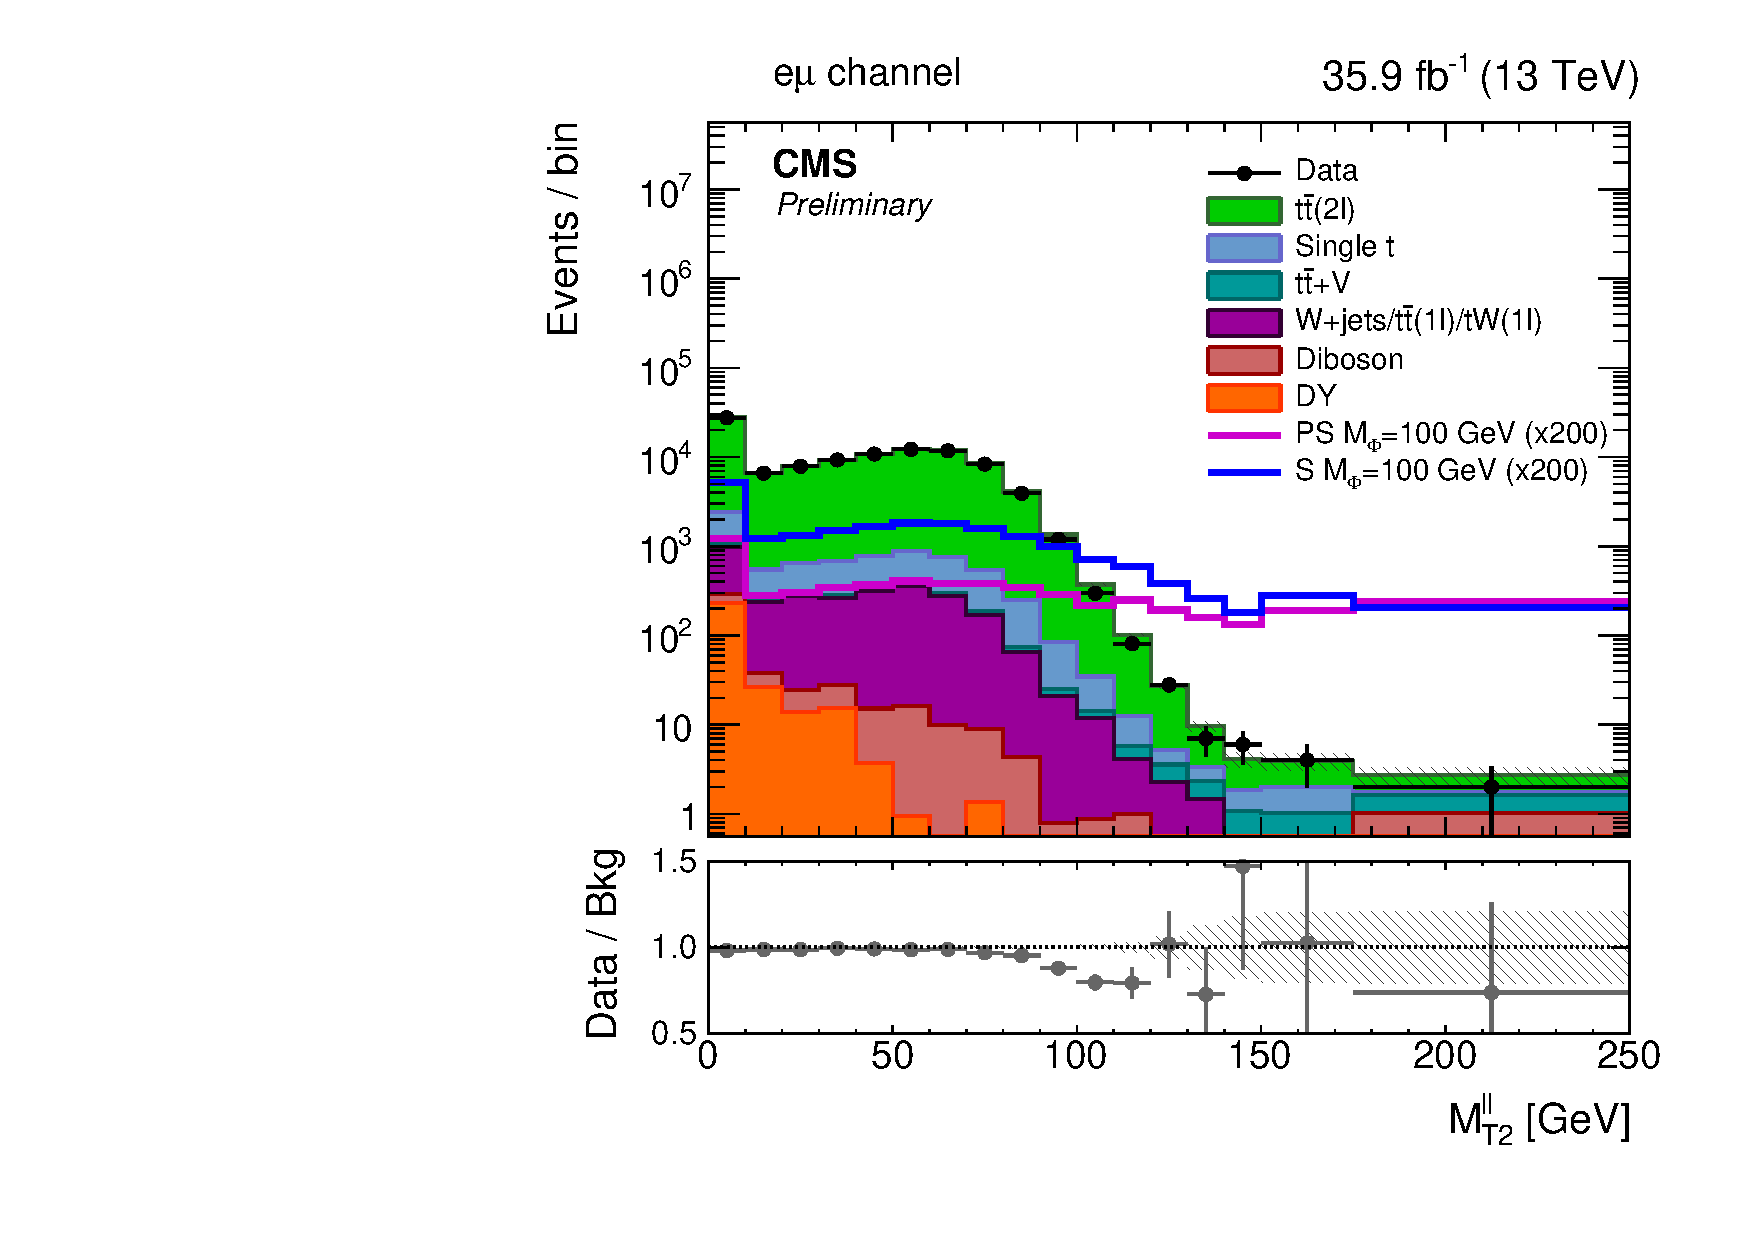
\includegraphics[width=0.6\textwidth]{figs/mt2log_em.pdf}
  \caption{The \mttll distribution in data and simulation for events passing selection requirements for the $e\mu$ channel. The distributions of two example signal models with S and PS mediators of $\mMed = 100\:\GeV$, and with $\mDM=1\:\GeV$ are also presented and scaled up by a factor of 200. The last bin in the distribution includes overflow, and the uncertainties are statistical only.}
  \label{fig:mt2ll}
\end{figure}


